%%
% TUM Corporate Design LaTeX Templates
% Based on the templates from https://www.tum.de/cd
%
% Feel free to join development on
% https://gitlab.lrz.de/tum-templates/templates
% and/or to create an issue in case of trouble.
%
% tum-article class for scientific articles, reports, exercise sheets, ...
%
%%

\documentclass[twocolumn]{tum-article}
%\documentclass[twocolumn, german]{tum-article}
%\documentclass[times, twocolumn]{tum-article}
%\documentclass[times]{tum-article}
%\documentclass{tum-article}

%\usepackage{lipsum}
\usepackage{amsmath}

\title{Analysis of the 2014 Passenger Flight Network}
\author{Felix Paul Niemeyer\authormark{1},
	Saicharan Kumar\authormark{2}}
% Author 3\authormark{1}\orcid{0000-0000-0000-0000}}

% if too long for running head
\titlerunning{TUM Article}
\authorrunning{Author 1 et al.}

%\email{niemeyer.felix@tum.de}

\affil[1]{felix.niemeyer@tum.de, MiM}
\affil[2]{saicharan.kumar@tum.de, MiM}

\date{Received: 19.02.2020 - This is work in progress}

% for the equation stuff 
\DeclareMathOperator{\avgFlow}{avgFlow}
\DeclareMathOperator{\patronage}{patronage}
\DeclareMathOperator{\flow}{flow}
\DeclareMathOperator{\weight}{weight}
\DeclareMathOperator{\PNWS}{PNWS}
\DeclareMathOperator{\NOE}{NOE}
\DeclareMathOperator{\degree}{degree}
\DeclareMathOperator{\flowSum}{flowSum}
\DeclareMathOperator{\flowDeviation}{flowDeviation}
\DeclareMathOperator{\flowDiff}{flowDiff}

\begin{document}

\maketitle

\begin{abstract}
In this case study we are looking at a dataset about air travel in 2014. 
We implement some mechanisms to clean the data, as well as mechanisms to enrich this dataset with information we query from wikidata.
We estimate some missing data.
Starting from there, we analyze some network characteristics for the whole network as well as airline-specific sub-networks.
We compare airline-specific networks and find relations between their network's characteristics and their business model.
We propose one metric that plays a role in forecasting whether a cooperation between two airlines is advantageous and use this metric to generate an alliances landscape.
We compare it's predictive correctness to the real world by looking at the formation of Vanilla Airlines which occurred in the year after the one our data stems from.
\end{abstract}

\section{Data Description}
The network analysis is based on dataset from openflights.org. 
It describes passenger flight connections between airports in the year 2014. 
The data includes, which airline each connection is operated by.
The data comes in three tables: airports, routes and airlines. 
The airports table has entries for every airport with the following useful information: \\
- airport id\\
- iata and icao codes\\
- geographic coordinates\\
- country and region\\

The routes table lists an entry for each connection between two airports that was operated by an airline sometime in the year 2014. It does not contain any information about flight frequencies or passenger volume. The airline table lists airlines associated with their name and some information we do not need like country or call sign. \\

We are loading these files into an SQLite database for easier handling. 
We apply some queries for cleaning the data, e.g. removing routes operated by unknown airlines or filling in airport ids in routes where only iata or icao code is used to refer to a source or destination airport. \\

All the data-setup can be accomplished by running a single script.
This script and also all other code we have written for this project can be found in a public repository on GitHub\cite{repository}.

\section{Data Enrichment \& Estimation}
After cleaning up the data, there are 3139 airports. 
Interpreting the data as a graph gives us a multi-edge directed graph).
Looking at the degree distribution in Figure~\ref{fig:degree_distribution}, the alternating characteristic of degrees strikes the eye. It comes from the fact, that it's very uncommon for a connection between airports to exist only in one direction. Thus, there is much fewer nodes with odd degrees than than with even degrees. 

When we disregard odd degrees, the seemingly linear distribution on a log log scale becomes apparent. Using least square (scipy.optimize.curve\_fit), we optimize parameters $c$ and $\gamma$ as you can see in Figure~\ref{fig:degree_distribution_curves}

\begin{figure}
	\centering
	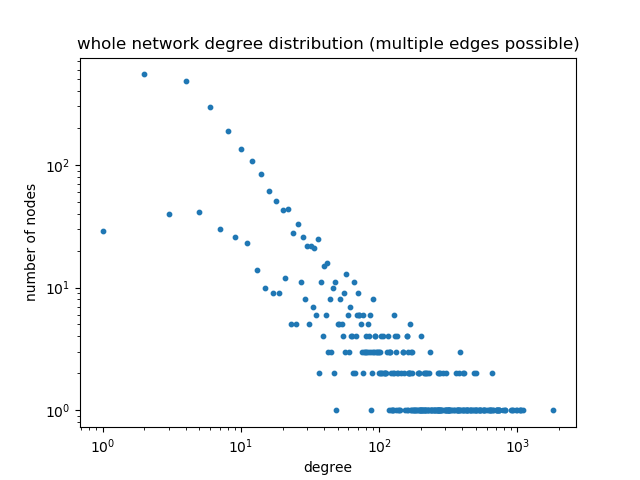
\includegraphics[width=76mm]{imgs/results/degree_distribution_incl_odd_degrees.png}
	\caption{
The degree distribution of the network on a log log scale }
	\label{fig:degree_distribution}
\end{figure}

\begin{figure}
	\centering
	\includegraphics[width=76mm]{imgs/results/degree_distribution_curve_manual.png}
	\caption{
Looking at even degrees only. Trying least square curve fitting to find suitable parameters for power law distribution function $f(x) = a * x^{-\gamma}$}
	\label{fig:degree_distribution_curves}
\end{figure}

Besides the main subgraph, that includes 3113 nodes, there are 6 small disconnected ones with only a couple of nodes.
One with 10 nodes for example Figure~\ref{fig:new_caledonia}, consists only of airports that are located in New Caledonia, an archipelago in the Pacific Ocean. 
\begin{figure}
	\centering
	\includegraphics[width=76mm]{imgs/new-caledonia-subgraph.png}
	\caption{Airports of New Caledonia drawn on a map}
	\label{fig:new_caledonia}
\end{figure}

In order to enable us to do more meaningful analysis, we enrich the dataset with additional information. We chose the airport patronage and found out, that we can get this data from Wikidata. 
For 1956 of the 3139 airports from the dataset, we can find patronage data from Wikidata. Get an impression about the regional differences of data availability by looking at the percentage of airports for which Wikidata yields a patronage in Table~\ref{tab:patr_av_most_airports} and Table~\ref{tab:patr_av_worst}.
\begin{table}[h]
	\centering
	\caption{patronage data availability on Wikidata for countries with the most airports}
	\label{tab:patr_av_most_airports}
	\begin{tabular}{|l|c|c|}
		\hline
		Country & Airports & patronage present \\ \hline
		United States & 539 & 34.1\%\\
		China & 173 & 95.4\%\\
		Canada & 142 & 48.6\%\\
		Brazil & 122 & 93.4\%\\
		Australia & 113 & 77.0\%\\
		Russia & 103 & 96.1\%\\
		India & 70 & 92.9\%\\
		Indonesia & 63 & 60.3\%\\
		Japan & 62 & 82.3\%\\
		Mexico & 56 & 92.9\%\\
		France & 55 & 96.4\%\\ \hline
	\end{tabular}
\end{table}
\begin{table}[h]
	\centering
	\caption{patronage data availability - worst countries}
	\label{tab:patr_av_worst}
	\begin{tabular}{|l|c|c|}
		\hline
		Country & Airports & patronage present \\ \hline
		Venezuela & 23 & 4.3\%\\
		Bahamas & 17 & 5.9\%\\
		Chile & 16 & 6.3\%\\
		Ecuador & 14 & 7.1\%\\
		Ethiopia & 13 & 7.7\%\\ 
		Mozambique & 10 & 10.0\%\\
		Cuba & 9 & 11.1\%\\
		Kenya & 16 & 12.5\%\\
		Namibia & 8 & 12.5\%\\
		Madagascar & 13 & 15.4\%\\
		Algeria & 26 & 19.2\%\\ \hline
	\end{tabular}
\end{table}
We need to distinguish between monthly and yearly values and we extrapolate 2014 data from close years in case no data for the year 2014. 
In order to populate the remaining nodes with reasonable patronages as well, we tried different techniques. 
First we used data about runway surfaces that we found on ourflights.org. 

We summed up the surfaces of runways for every airport and then calculated the average ratio between total runway surface area and patronage of airports where both data points were present, in order to predict patronage for airports without patronage data but with runway surface data based on this average ratio. For the still remaining >1000 airports without patronage we would then apply a default value that equals the average of the smallest 1\% of airports with patronage data from Wikidata. 
The runway data turned out to be very unclean and unreliably. Water runways and other quirks were distorting the predictions. 

Inspired by Prof. Ikonnikova advice during the presentation we switched to estimating the remaining airport patronages by looking at neighboring airports with patronage data. The Algorithm can be seen in Listing~\ref{lst:patronage_estimation_algorithm}.
\begin{lstlisting}[language=Python, caption={Patronage estimation algorithm, that using neighboring airport's patronage data}, label=lst:patronage_estimation_algorithm]
G = loadEntireNetwork()
pr = -1 #previous remaining
r = 0   #remaining
while r != pr:
  pr = r
  r = 0
  ep = {} #estimated patronages
  for apid in G.nodes:
    node = G.nodes[apid]
    if node["patronage"] == None:
      neighbors = G.neighbors(apid) 
      deg = G.degree(apid)
      sum = 0
      count = 0
      for nid in neighbors: 
        n = G.nodes[nid]
        npatr = n["patronage"]
        ndeg = G.degree(nid) 
        if npatr != None: 
          sum += deg * npatr / ndeg
          count += 1
      if count == 0:
        r += 1
      else:
        avg = sum / count
        ep[apid] = avg 
  for apid in ep: 
    node = G.nodes[apid]
    node["patronage"] = ep[apid]
\end{lstlisting}
This second approach yields much nicer estimations, as we will see after estimating the flows between airports. 

After estimating missing patronage data by looking at neighboring airports patronages, 14 airports without patronage remain. These must be in airports in disconnected subgraphs, because the algorithm would eventually reach them and assign a patronage otherwise. Investigations confirm that. We disregard these few dataless airports from disconnected subgraphs in the following analyses and thus end up with a network of 3125 airports. 

The flows are estimated by choosing reasonable initial values and then applying corrections iteratively to approach a situation where the sum of the estimated flows for each airport equal its patronage value.
The average initial values for an edge between airport $p$ and $q$ is chosen as: 


\begin{equation}
\avgFlow(pq) = \dfrac{\patronage(p) * \patronage(q)}{\degree(p) * \degree(q)}
\end{equation}
Remember that we are handling a multi-edge directed graph here. 
\begin{equation}
E = \{(pql) | \exists\ \text{route from}\ p\ \text{to}\ q\ \text{by}\ l\}
\end{equation}
where $p$ and $q$ are airports and $l$ is an airline.
Let us introduce a function $E(pq)$ that returns all edges between $p$ and $q$ disregarding the direction and operating airline. 
\begin{equation}
E(pq) = \{pql | \exists_{l \in L}:pql \in E \lor qpl \in E\}
\end{equation}
where $L$ is the set of airlines.

And let us introduce the function $E(p)$ that returns all edges from and to an airport $p$ by every airline: 
\begin{equation}
E(p) = \{rsl | (r=p \lor s=p) \land \exists_{l \in L}:rsl \in E \}
\end{equation}
The Edges of the graph are thus triplets of a source airport, destination airport and an airline.
There may be multiple edges between two airports pointing in different directions and/or operated by different airlines.
We could assume an equal distribution of the flows among the edges. But we chose trying to be closer to reality by weighting the flow of an edge between two airports $p$ and $q$, that is operated by airline $l$, by the geometric mean of the number of edges airline $l$ operates at airport $p$ and number of edges airline $l$ operates at airport $q$: 
\begin{equation}
\begin{aligned}
&\flow(pql) =\\
={}&\avgFlow(pq)  
* \NOE(pq) 
* \weight(pql) 
\end{aligned}
\end{equation}
where $\NOE(pq)$ is the number of edges between airport $p$ and $q$ and $\weight(pql)$ is defined as follows: 
\begin{equation}
\begin{aligned}
&\weight(pql) = \dfrac{\sqrt{\degree_{l}(p) * \degree_{l}(q)}}{\PNWS(pql)}
\end{aligned}
\end{equation}
where the $\PNWS(pq)$ (Pre Normalization Weight Sum) is just the sum of the non-normalized weights of all the routes from different airlines used to normalize the weights. 
\begin{equation}
\begin{aligned}
&\PNWS(pq) = \\
={}&\displaystyle\sum_{rsm \in E(pq)}(\sqrt{\degree_{m}(r) * \degree_{m}(s)})
\end{aligned}
\end{equation}
where $\degree_l(p)$ is the degree of airport $p$ in airline $l$'s subgraph, i.e. number of edges from and to airport $p$ operated by airline $l$.

The ratios we choose here will stay intact over the course of the iterations in the next part of the algorithm.
In every iteration, we traverse all airports and for every airport we calculate the sum of current flows values of all routes. 
\begin{equation}
\begin{aligned}
\flowSum(p) = \displaystyle\sum_{pql \in E \cup pu \in E}\flow_{pql}
\end{aligned}
\end{equation}
Difference between the patronage and the current sum of passenger flows of incoming and outgoing routes. 
Then, for each airport we calculate the difference between its patronage and the current sum of flows.
\begin{equation}
\begin{aligned}
\flowDiff(p) = \patronage(p) - \flowSum(p) 
\end{aligned}
\end{equation}
With this information given, we can now calculate for every edge $pql$ the change in its flow. 
\begin{equation}
\begin{aligned}
\forall_{pql \in E(p)}: & \\
& \Delta \flow(pql) = & \\ 
& ={} \dfrac{\flow(pql)}{\flowSum(p)}\flowDiff(p) \\
& +{} \dfrac{\flow(pql)}{\flowSum(q)}\flowDiff(q) \\
\end{aligned}
\end{equation}
and the more perfect flows for the edges and starting point for the next itaration are
\begin{equation}
\begin{aligned}
\forall_{pql \in E(p)}: & \\
& \flow'(pql) = \flow_{abo} + \Delta \flow(pql)
\end{aligned}
\end{equation}

In order to look at the results of this algorithm we introduce a measure 
\begin{equation}
\flowDeviation(p) = ln\left(\dfrac{\flowSum(p)}{\patronage(p)}\right)
\end{equation}
it expresses how well the sum of estimated flows match the patronage, that we know for the airport. If the flows are half the patronage the absolute value of $\flowDeviation$ will be the same as when the current flows are twice the actual patronage number. 
We compare the results between estimating the patronages based on the runway sizes Figure~\ref{fig:flow_deviation_runway} and estimating the patronages based on neighboring airports Figure~\ref{fig:flow_deviation}. 
The blue line shows the $\flowDeviation$ distribution of the initial flow values.
The other lines show the $\flowDeviation$ distribution after a the first couple of iterations and after the final iteration. 
In the case of patronage estimations based on neighboring airports, we see that the $\flowDeviation$ distribution after the 120th iteration comes very close to $y=0$ which is also reflected by the $sum(abs)$ in the legend which is the sum of the absolute value of $\flowDeviation$ over all airports which is $0.94$ in this case.

The bad results of the estimations when estimating patronage values from runways stem from constellations like in Figure~\ref{fig:impossible_flows}, when choosing flows to match the patronage values are impossible. 
The constellation that accounts for $>0.88$ of the $\flowDeviation$ sum $0.94$ in the scenario where patronages are estimated based on neighboring airports is shown in Figure~\ref{fig:worst_flow_fit}. 
The patronage of both airports comes from Wikidata. After further investigation it turns out to be probable, that there should be a connection between Arvidsjaur Airport and Stockholm-Arlanda Airport, which is not present in the data set. 

\begin{figure}[h]
	\centering
	\includegraphics[width=76mm]{imgs/flow_estimation_runway_approach_deviation.png}
	\caption{
Estimated flows when estimating patronage based on the runway size and a default value}
	\label{fig:flow_deviation_runway}
\end{figure}

\begin{figure}[h]
	\centering
	\includegraphics[width=76mm]{imgs/results/flow_estimation_120_iterations.png}
	\caption{
Estimated flows when estimating patronage based on neighboring airport's patronage}
	\label{fig:flow_deviation}
\end{figure}

The complete algorithm for passenger flow estimation can be found in the repository: ./scripts/estimate-passenger-flows.py

\begin{figure}[h]
	\centering
	\includegraphics[width=76mm]{imgs/runway-based-estimation-problem.png}
	\caption{Worst situation in the scenario, where patronages are estimated based on runways and a default value: 
For Qaanaaq Airport there was no patronage data from Wikidata and no runway information. That's why it ended up with the default patronage value 1523. In this constallation it is impossible to choose passenger flows that even remotely satisfy the the patronages of airports with ids 10 and 5446}
	\label{fig:impossible_flows}
\end{figure}

\begin{figure}[h]

	\centering
	\includegraphics[width=76mm]{imgs/results/ego_graph_730.png}
	\caption{Worst situation in the scenario, where patronage is based on neighboring airport's patronage: 
Arvidsjaur Airport is only connected to Lycksele Airport but has a more than twice as high patronage than Lycksele Airport}
	\label{fig:worst_flow_fit}
\end{figure}



\section{Basic Network Analysis}
Initially, we would like to analyse the entire worldwide airline network, and provide some insights regarding the airline industry.
Since a particular route could be provided by multiple Airline Companies, the final network that we come up with is a Multiple Directed Network.
The attributes of each edge in this network included both the geometrical distance and the average passenger flow of that route (edge). 
As we can see from the Table~\ref{Tab:distance_metrics}, the diameter of the entire network is given along with the Total Distance of the routes and the Average Distance of routes in a network.  

\begin{center}
\begin{table}[ht]	
 \begin{tabular}{| c | c | c |}
 \hline
 \textbf{Diameter (km)} & \textbf{Total Dist.(km)} & \textbf{Average Dist.(km)} \\ [0.5ex]
 \hline
 18834 & 126681574 & 1889.72 \\
 \hline
 \end{tabular}
\caption{Distance Metrics of the Network}
\label{Tab:distance_metrics}	 
\end{table}
\end{center}

We currently do not have the ability to calculate centrality parameters like Eigenvector, Closeness or Betweenness Centrality for a Multidirected Graph. So we will be mainly looking at Degree Centrality of the entire network as shown in Figure~\ref{fig:degree_centrality}.
This is because Degree Centrality is the only Centrality available for Multiple Directed Graphs.

\begin{figure}
        \centering
        \includegraphics[width=80mm]{imgs2/results/degree_centrality_whole_network.png}
        \caption{
The degree centrality of the entire network}
        \label{fig:degree_centrality}
\end{figure}

The degree centrality is given by the formula:
\begin{equation}
	Degree Centrality=d_i/(n-1)
\end{equation}

Just by analysing the graph, we can say that the degree centrality distributrion is following the Power Law Distribution.

\section{Airline Subgraph Analysis \& Comparison}

Airline Networks can be mainly divided into two different types of networks. Full Service Airlines which are also called as Legacy Carriers, and Low Cost Airlines or Low Cost Carriers.  
Full Service Airlines generally provide free baggage allowance, meals, drinks, seat selection and in-flight entertainment at no extra charge.
Low Cost Carriers will usually collect ancillary revenue for all or most of the above these amentities.
Most of the time, Low Cost Carriers operate in a specific regions.
These specific regions could be within countries, or within continents, or within specific part of the continents.

\begin{figure}
        \centering
        \includegraphics[width=80mm]{imgs2/united_airline_network.png}
        \caption{
Network of United Airlines}
        \label{fig:united_airline}
\end{figure}

\begin{figure}
        \centering
        \includegraphics[width=80mm]{imgs2/american_airline_network.png}
        \caption{
Network of American Airlines}
        \label{fig:american_airline}
\end{figure}



Long haul low cost carriers are provided by very few carriers in the world, as it is not feasible to offer long routes with low cost and also high frequency, according to Robert L. Candall, former CEO of American Airlines.\cite{long_haul_lcc_model}
The only example we have of a long haul low cost carrier is Norwegian Airlines, as they offer flights from Scandinavia to different cities in the United States.
But this is more an exception, than the norm. For the long haul low cost carriers to survive and adapt, they must continue to innovate. Their business models should focus on three new emerging carrier types: Network, Product and Price Specialist, according to John G.Wensveen and Ryan Leick.\cite{long_haul_lcc_new_model}

Before we look at the differences in the network parameters of these two types of airlines, there are major differences in the network architecture itself.
While the major Full Service Airlines often have the Network Type of "Hub and Spoke", the Low Cost Carriers are known to have Point to Point Network Type, according to research by Cook G.N and Goodwin, J.\cite{airline_network_comparison}
This "Hub and Spoke" network connection can be seen in the network graph of United Airlines and American Airlines given in Figure~\ref{fig:united_airline} and Figure~\ref{fig:american_airline} respectively. These two airlines are prime example of Full Service Airlines. 

Similarly we see the "Point to Point" Network in Low Cost Carriers like Ryan Air in Figure~\ref{fig:ryan_air} and Southwest Airlines in Figure~\ref{fig:southwest_airline}.

\begin{figure}
        \centering
        \includegraphics[width=80mm]{imgs2/ryan_air_network.png}
        \caption{
Network of Ryan Air}
        \label{fig:ryan_air}
\end{figure}

\begin{figure}
        \centering
        \includegraphics[width=80mm]{imgs2/southwest_airline_network.png}
        \caption{
Network of Southwest Airlines}
        \label{fig:southwest_airline}
\end{figure}

\begin{table}[ht]
\begin{center}
 \begin{tabular}{| c | c |}
 \hline
 \textbf{Airline} & \textbf{Diameter (km)} \\ [0.5ex]
 \hline
 United Airlines & 12979 \\
 \hline
 American Airlines & 14076 \\
 \hline
 Delta Airlines & 13581 \\
 \hline
 Ryan Air & 3698 \\
 \hline
 Southwest Airlines & 3757 \\
 \hline
 Air Asia & 2914 \\
 \hline
 China Southern & 11637 \\
 \hline
 China Eastern & 11896 \\
 \hline
 \end{tabular}
\caption{Diameter of Major Airlines}
\label{Tab:diameter_metrics}
\end{center}
\end{table}



\begin{table}[ht]
\begin{center}
 \begin{tabular}{| c | c | c |}
 \hline
 \textbf{Airline} & \textbf{Mean (km)} & \textbf{Median (km)} \\ [0.5ex]
 \hline
 United Airlines & 2353.69 & 1393 \\
 \hline
 American Airlines & 2321.23 & 1371 \\
 \hline
 Delta Airlines & 2352.17 & 1341 \\
 \hline
 Ryan Air & 1490.21 & 1435.5 \\
 \hline
 Southwest Airlines & 1398.37 & 1267 \\
 \hline
 Air Asia & 1328.57 & 1254 \\
 \hline
 China Southern & 1459.95 & 1127 \\
 \hline
 China Eastern & 1427.81 & 1075 \\
 \hline
 \end{tabular}
\caption{Distance Metrics of Major Airlines}
\label{Tab:distance_airlines}
\end{center}
\end{table}


\begin{table}[ht]
\begin{center}
 \begin{tabular}{| c | c | c |}
 \hline
 \textbf{Airline} & \textbf{Mean Flow} & \textbf{Median Flow} \\ [0.5ex]
 \hline
 United Airlines & 85159 & 43286 \\
 \hline
 American Airlines & 67983.40 & 47185 \\
 \hline
 Delta Airlines & 76345.95  & 47123 \\
 \hline
 Ryan Air & 31268.60 & 26857.50 \\
 \hline
 Southwest Airlines & 65692.70  & 61590 \\
 \hline
 China Southern & 53100  & 43729.50 \\
 \hline
 China Eastern & 52610.60  & 43294 \\
 \hline
 \end{tabular}
\caption{Passenger Flow of Major Airlines}
\label{Tab:passenger_flow_airlines}
\end{center}
\end{table}

\begin{figure}
        \centering
        \includegraphics[width=80mm]{imgs2/results/united_eigenvalue_centrality.png}
        \caption{
Eigenvalue Centrality of United Airlines}
        \label{fig:united_air_ec}
\end{figure}

\begin{figure}
        \centering
        \includegraphics[width=80mm]{imgs2/results/delta_eigenvalue_centrality.png}
        \caption{
Eigenvalue Centrality of Delta Airlines}
        \label{fig:delta_air_ec}
\end{figure}


\begin{figure}
        \centering
        \includegraphics[width=80mm]{imgs2/results/american_eigenvalue_centrality.png}
        \caption{
Eigenvalue Centrality of American Airlines}
        \label{fig:american_air_ec}
\end{figure}


\begin{figure}
        \centering
        \includegraphics[width=80mm]{imgs2/results/ryan_eigenvalue_centrality.png}
        \caption{
Eigenvalue Centrality of Ryan Air}
        \label{fig:ryan_air_ec}
\end{figure}


\begin{figure}
        \centering
        \includegraphics[width=80mm]{imgs2/results/southwest_eigenvalue_centrality.png}
        \caption{
Eigenvalue Centrality of Southwest Airlines}
        \label{fig:southwest_air_ec}
\end{figure}


\begin{figure}
        \centering
        \includegraphics[width=80mm]{imgs2/results/chinasouthern_eigenvalue_centrality.png}
        \caption{
Eigenvalue Centrality of China Southern Airlines}
        \label{fig:chinasouthern_air_ec}
\end{figure}


\begin{figure}
        \centering
        \includegraphics[width=80mm]{imgs2/results/chinaeastern_eigenvalue_centrality.png}
        \caption{
Eigenvalue Centrality of China Eastern Airlines}
        \label{fig:chinaeastern_air_ec}
\end{figure}


\section{Airline Cooperation Opportunity}

The possibility to provide convenient on-line connections to clients is an important factor that drives welfare gains through airline cooperation according to E. E. Bailey and D. Liu \cite{airline_consolidation_and_consumer_welfare}.

\section{Reality Check: Vanilla Airlines}


\section*{Acknowledgments}


\bibliographystyle{IEEEtran}
\bibliography{literature}

\end{document}
